% Chapter 4 — Results & Analysis

\chapter{Results \& Analysis}

\label{Chapter4}

\section{Parameter Identification on the Optimization Experiment}
\label{sec:results-identification}

The two-stage optimizer of Section~\ref{sec:identification} identified the six
parameters for all ten cells from the loaded window of the Optimization
Experiment. The complete set of tuned values is given in
Appendix~\ref{app:tables}, Table~\ref{tab:params-opt}. For the healthy cells the
calibration RMSE ranges from 2.0 to 11.3\,mV --- below 12\,mV in every case --- and
the mean time-series RMSE over the healthy cells is 8.0\,mV. These figures confirm
that a six-parameter law reproduces each cell to within a few millivolts.

Figure~\ref{fig:ts-opt-stack} places the experiment in context. The stack sits at
its open-circuit plateau of about 4.57\,V, drops to roughly 0.8\,V when the
$25\,\Omega$ resistor is connected at $t=135$\,s, draws a load current that decays
from about 30\,mA, and recovers when the resistor is removed at $t=684$\,s. The
simulated stack voltage (sum of the ten calibrated cells) tracks the measured
trace throughout the loaded window, which shows that the per-cell fits aggregate
correctly to the stack level.

\begin{figure}[t]
    \centering
    
\includegraphics[width=0.92\linewidth]{Figures/comparison_exp19_stack.png}
    \caption[Stack voltage and load current, Optimization Experiment]{Stack
             voltage and load current during the Optimization Experiment.
             \textbf{Top:} measured (blue) and simulated (red) stack voltage; the
             load is applied at $t=135$\,s and removed at $t=684$\,s.
             \textbf{Bottom:} the load current $I=V_{\text{stack}}/25\,\Omega$.
             The close overlap in the loaded window confirms that the calibrated
             cell models sum to the correct stack voltage.}
    \label{fig:ts-opt-stack}
\end{figure}

\begin{figure}[t]
    \centering
    
\includegraphics[width=\linewidth]{Figures/all_cells_overview_exp19.png}
    \caption[Per-cell voltage--current calibration fits]{Per-cell
             voltage--current calibration fits: measured points (blue) versus the
             identified model (red). The seven healthy cells (3--9) are matched
             with RMSE between 2.0 and 11.3\,mV. Cells~0--2 (highlighted) collapse
             to a near-zero voltage under load, so the optimizer cannot produce a
             meaningful curve --- a clear signature of hardware degradation.}
    \label{fig:vi-opt}
\end{figure}

The per-cell calibration fits in Figure~\ref{fig:vi-opt} explain these numbers.
Two findings stand out. First, the model describes the healthy cells accurately
with only six parameters: the activation coefficients are consistent across cells,
while the concentration ($B$) and contact-resistance ($c$) terms stay close to
zero, indicating that activation and ohmic effects dominate over the covered
range. Second, the identification doubles as a \emph{diagnosis} tool. Cells~0, 1,
and~2 collapse to about 0\,V under load, and the optimizer returns identical,
degenerate parameter sets for them (RMSE below 0.1\,mV against a flat near-zero
signal). This is the signature of a non-functioning electrode, not a physically
meaningful fit, because no parameter combination within the bounds can reproduce a
dead cell.

The time-series comparison in Figure~\ref{fig:ts-opt-cells} confirms the fit cell
by cell. The simulated voltage overlays the measurement for the healthy cells
across the loaded window, whereas Cells~0--2 remain pinned near zero. The slightly
larger residuals of Cells~7 and~9 stem from the load-on transient, which the
calibration window deliberately excludes; over the settled window the agreement is
within the reported RMSE.

\begin{figure}[t]
    \centering
    
\includegraphics[width=\linewidth]{Figures/comparison_exp19_cells.png}
    \caption[Per-cell voltage: measured vs.\ simulated]{Per-cell voltage,
             measured (blue) versus simulated (red), over the full experiment.
             Healthy cells (3--9) are tracked closely; the degraded cells~0--2
             stay near zero under load. Titles report the time-series RMSE over
             the loaded window (mean 8.0\,mV for the healthy cells).}
    \label{fig:ts-opt-cells}
\end{figure}

\section{Step-Response Characterization (TR-Current Experiments)}
\label{sec:results-tr}

The TR-current experiments characterize how fast the stack current settles after a
load step. In both runs, Cells~1 and~2 read about 0\,mV throughout the loaded
window, confirming the degradation first seen in the Optimization Experiment; the
other cells behave normally. Figure~\ref{fig:tr-experiments} shows the raw
channels for the two loads.

\begin{figure}[t]
    \centering
    \begin{subfigure}[t]{0.49\linewidth}
        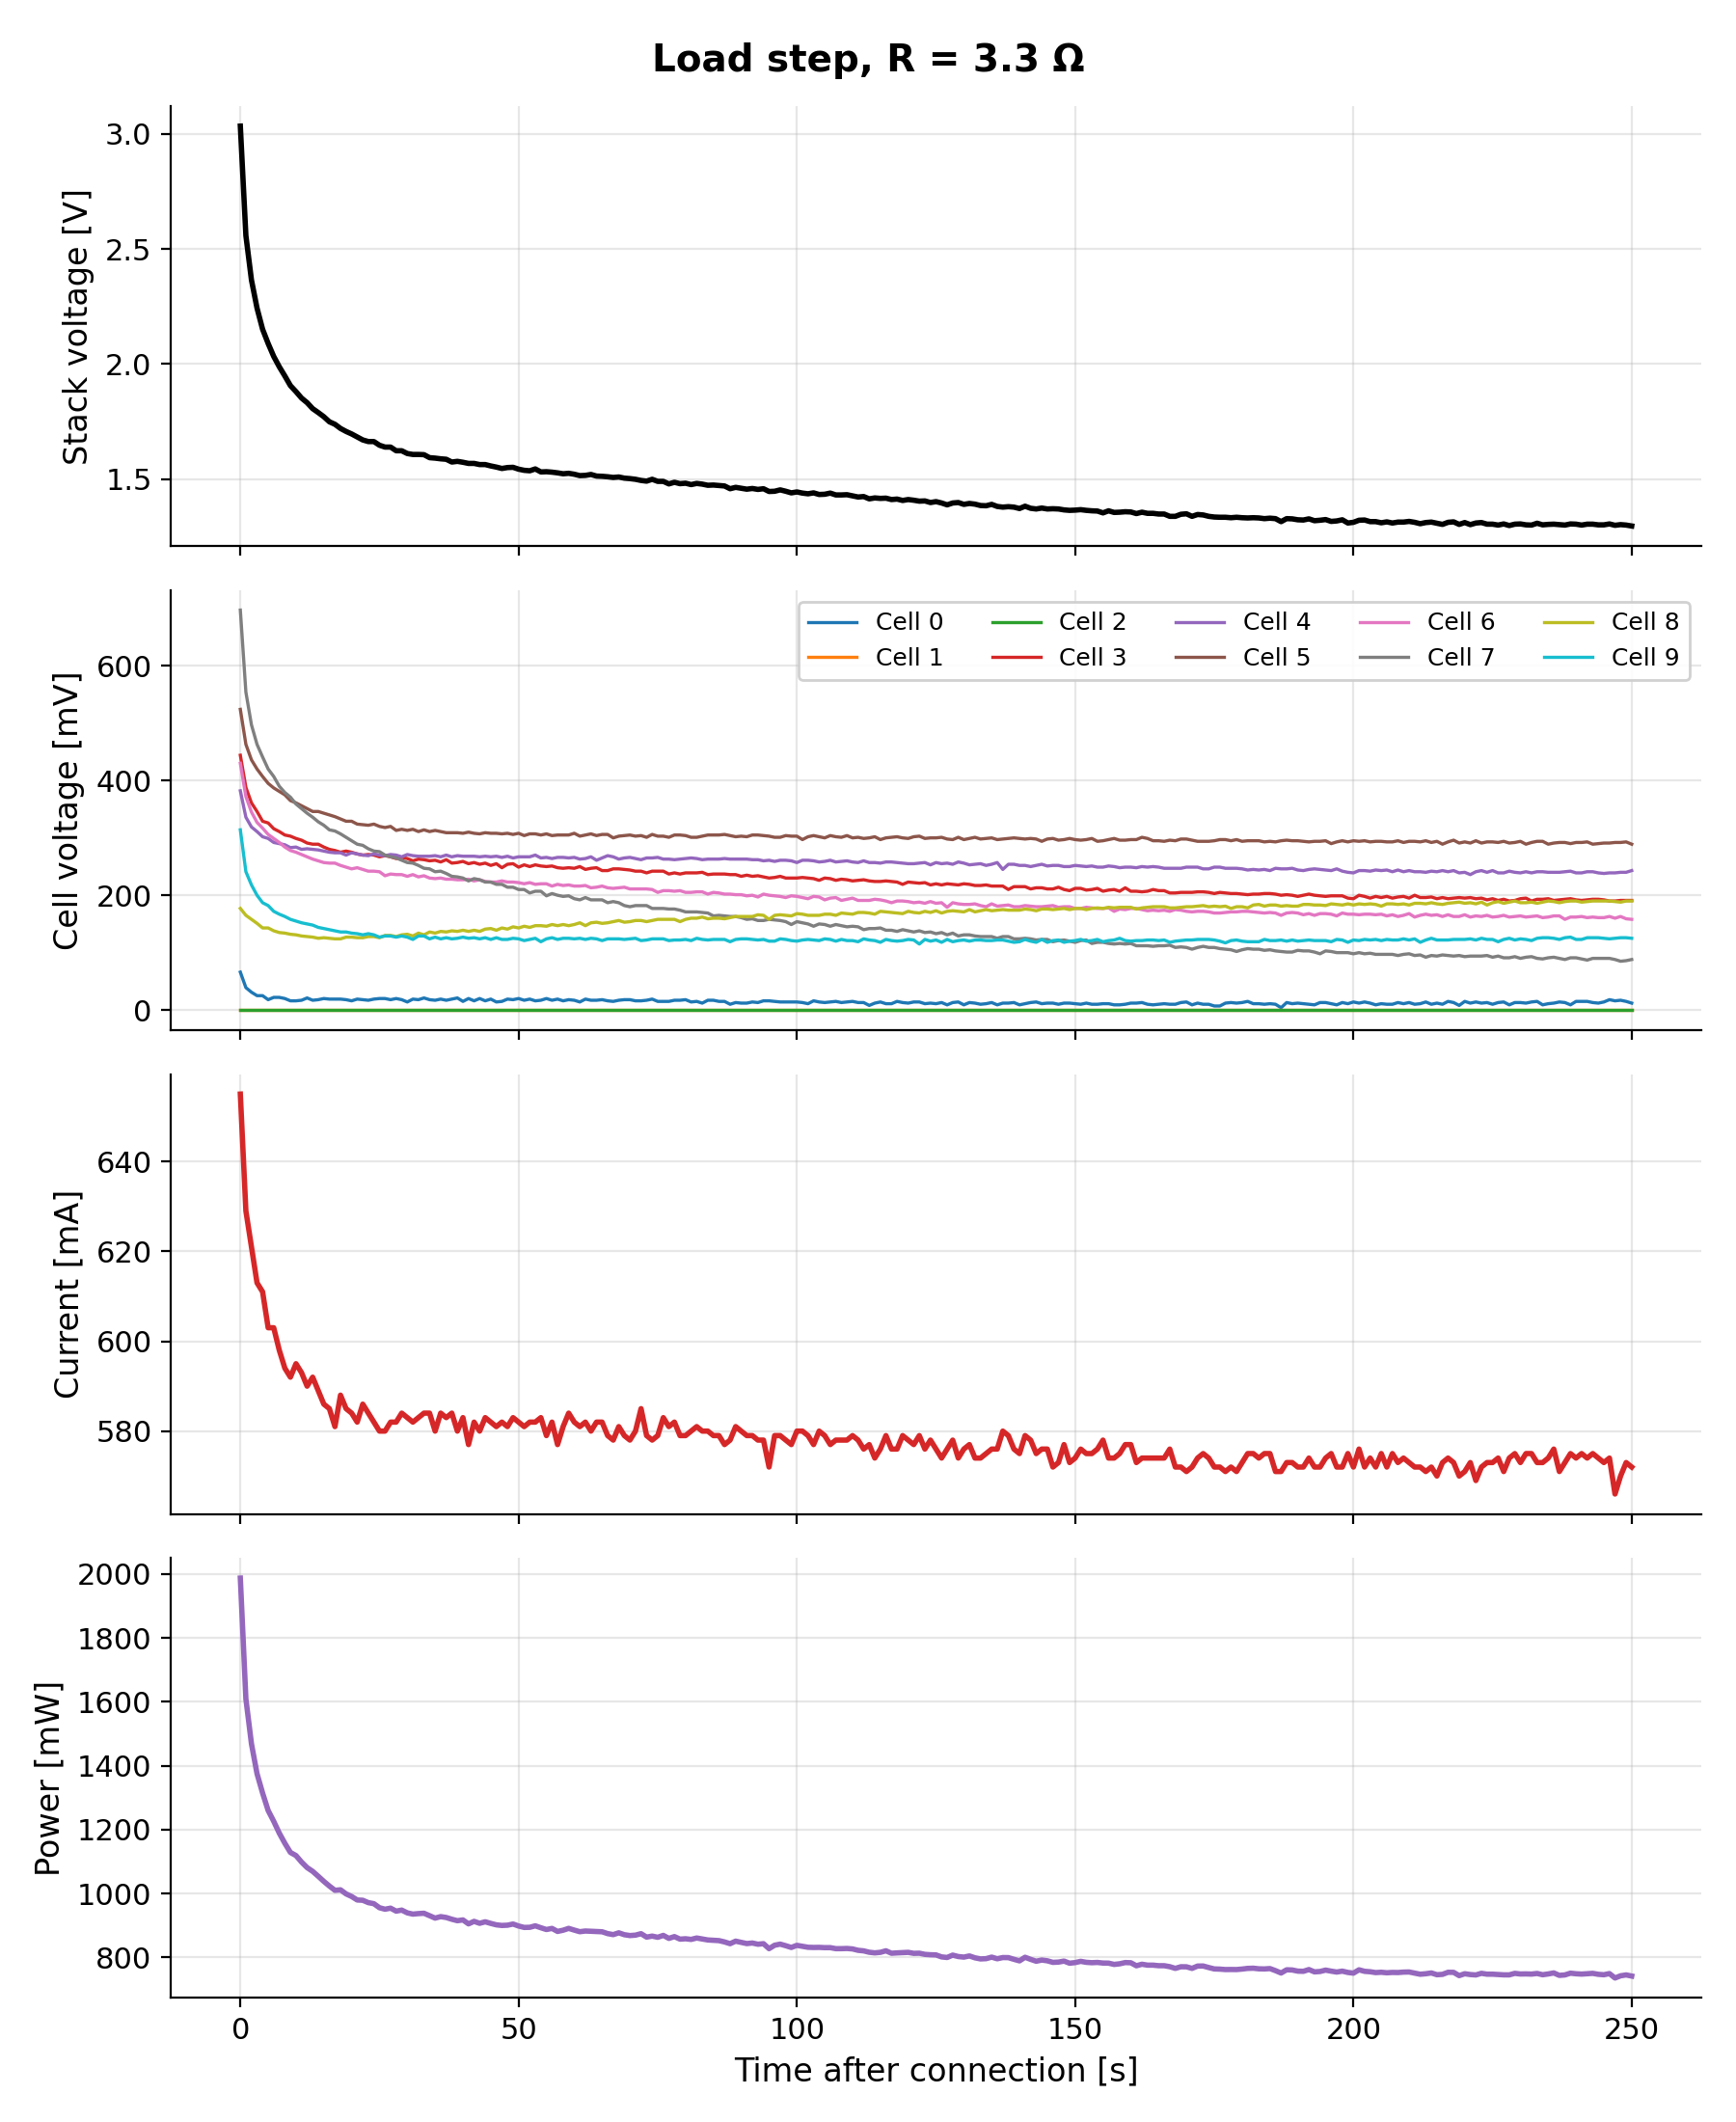
\includegraphics[width=\linewidth]{Figures/exp_33ohm_plot.png}
        \caption{Experiment~1, $R=3.3\,\Omega$.}
    \end{subfigure}\hfill
    \begin{subfigure}[t]{0.49\linewidth}
        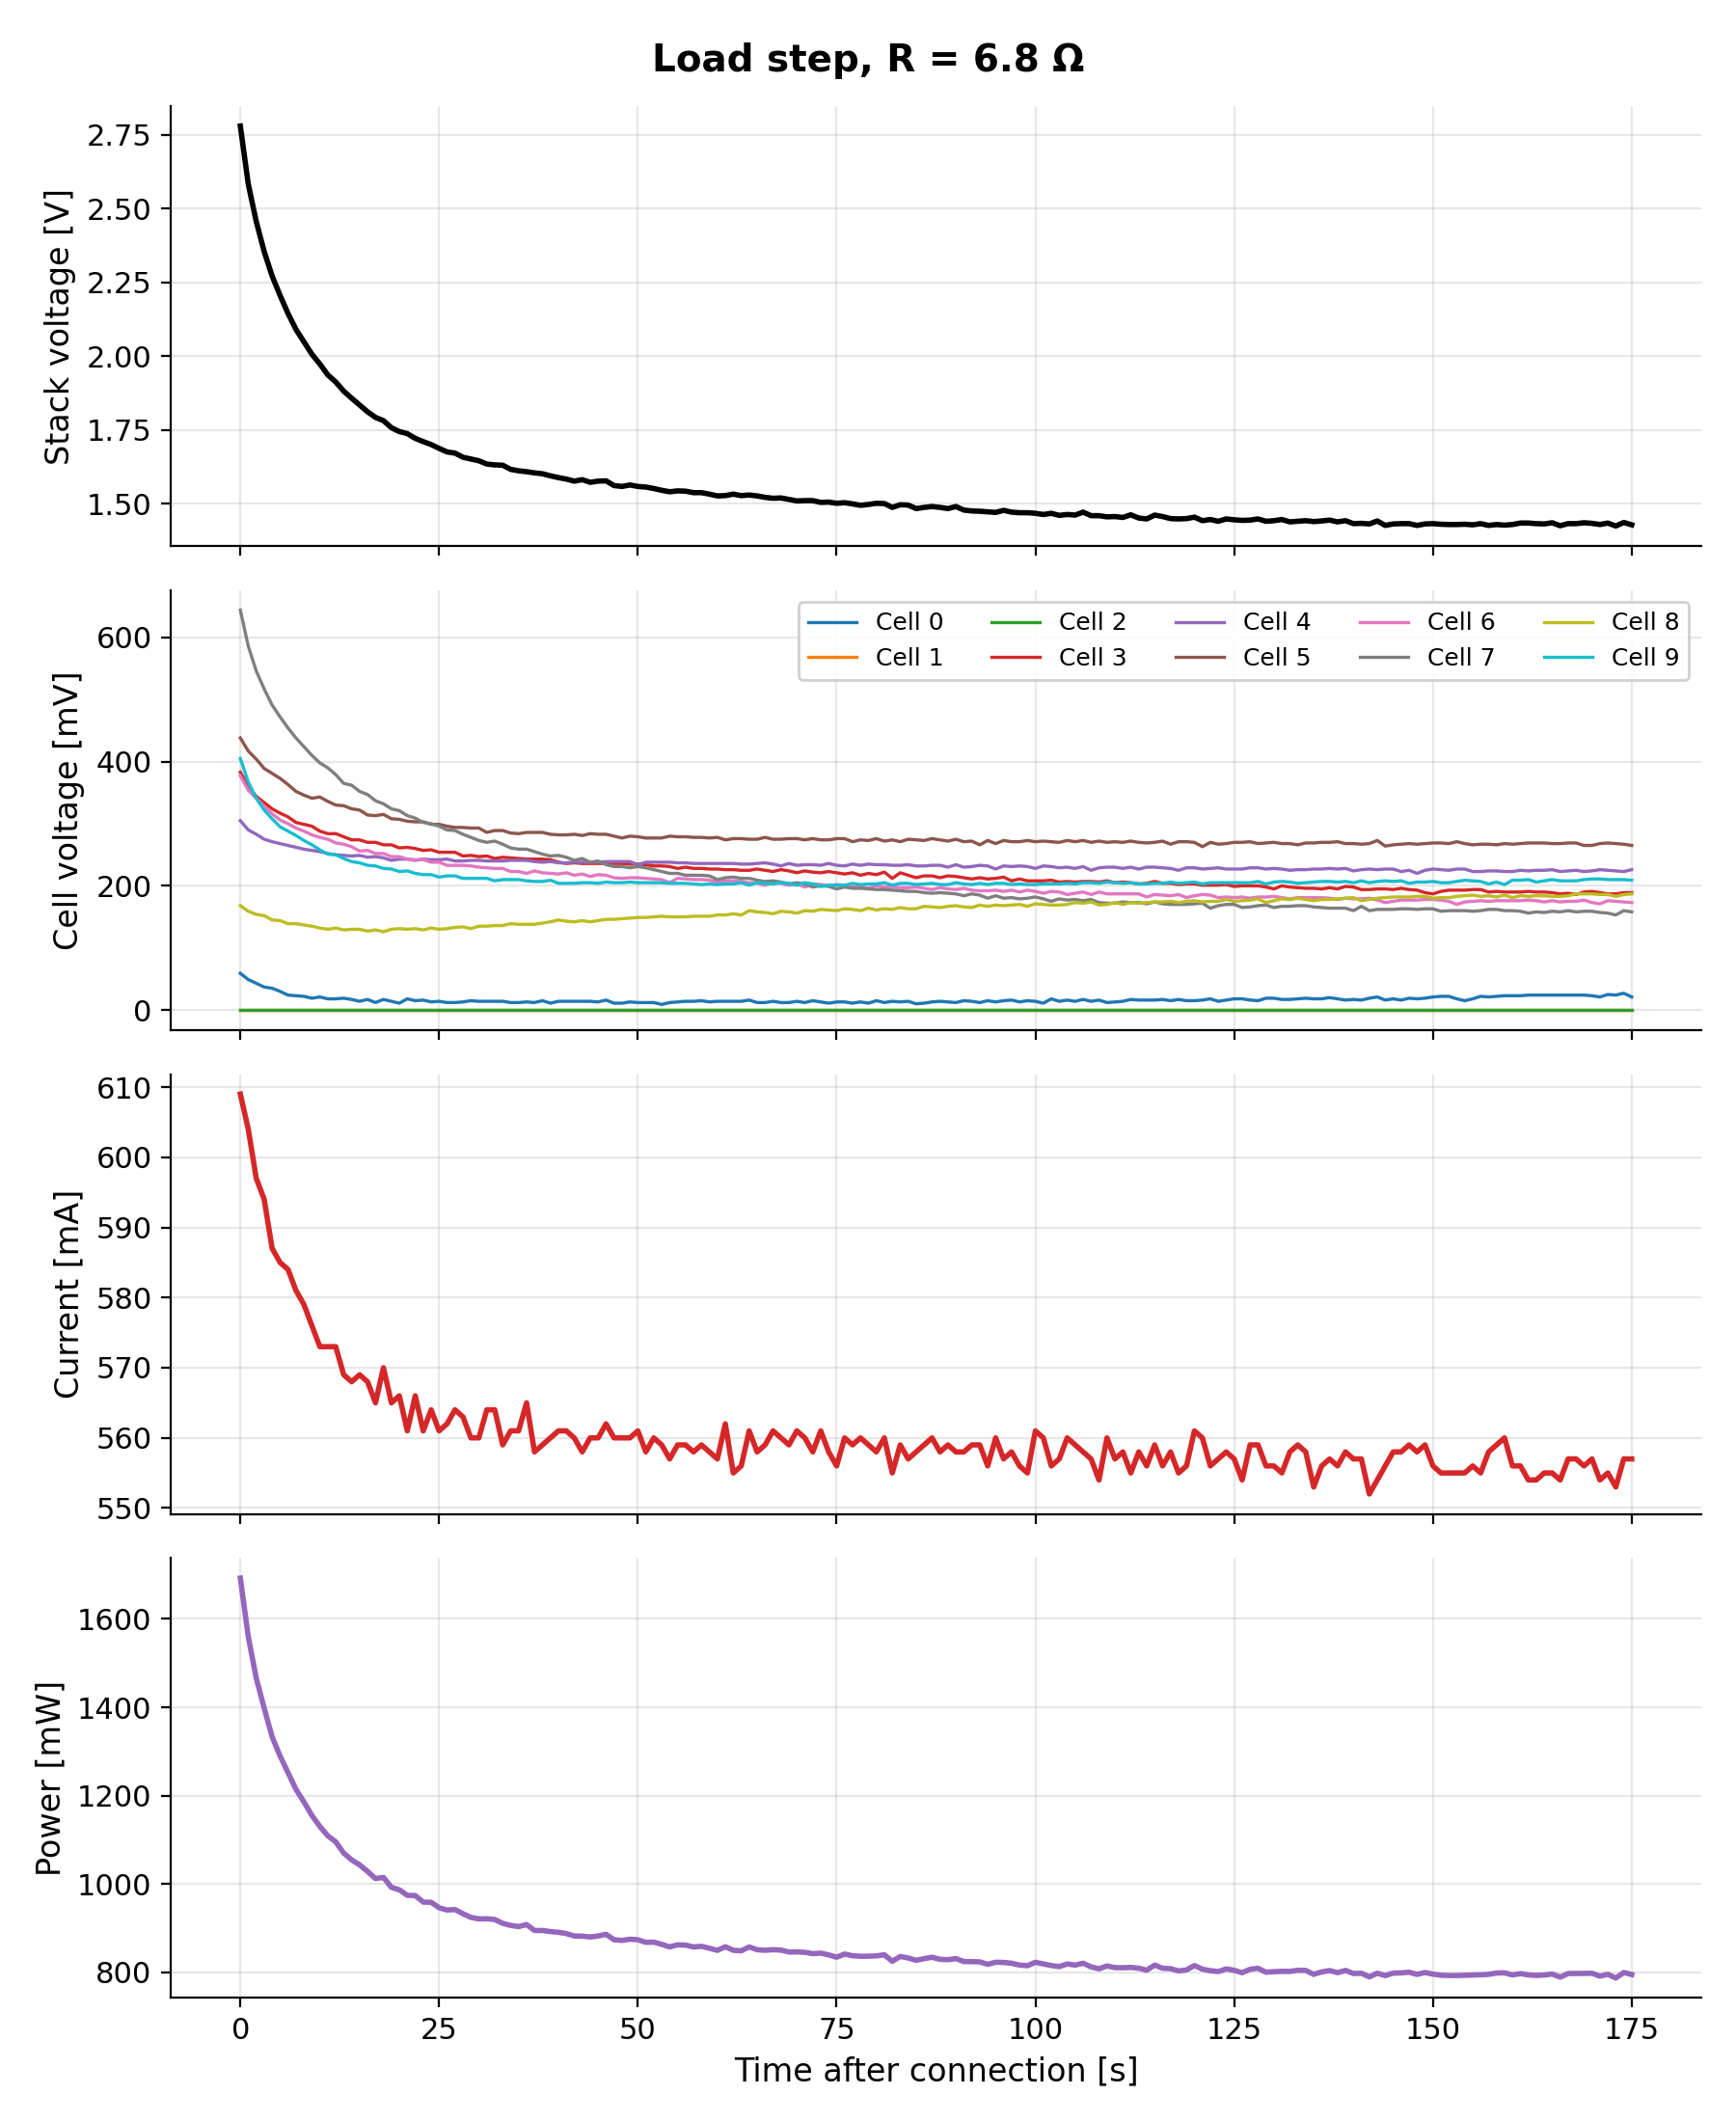
\includegraphics[width=\linewidth]{Figures/exp_68ohm_plot.png}
        \caption{Experiment~4, $R=6.8\,\Omega$.}
    \end{subfigure}
    \caption[TR-current step experiments]{TR-current step experiments after
             resistor connection (time re-zeroed to the step): stack voltage,
             individual cell voltages, current, and power. Both signals relax
             monotonically toward a steady state, with no overshoot --- behavior
             well captured by a first-order model.}
    \label{fig:tr-experiments}
\end{figure}

Fitting the first-order model $I(t)=I_{\text{ss}}+\Delta I\,e^{-t/\tau_I}$ to the
current gives the metrics of Table~\ref{tab:response-rt}, illustrated in
Figure~\ref{fig:tr-responses}.

\begin{table}[H]
    \centering
    \caption[Current step-response metrics]{Current step-response metrics for the
             two loads. The lighter load ($6.8\,\Omega$) gives a longer time
             constant and a smaller initial perturbation, consistent with slower
             dynamics at lower current density.}
    \label{tab:response-rt}
    \small
    \begin{tabular}{lcc}
        \toprule
        \textbf{Current metric} & \textbf{Exp~1 (3.3\,$\Omega$)} & \textbf{Exp~4 (6.8\,$\Omega$)} \\
        \midrule
        Steady-state current $I_{\text{ss}}$ [mA] & 572.9 & 556.1 \\
        Step amplitude $\Delta I$ [mA]             &  82.1 &  52.9 \\
        Time constant $\tau_I$ [s]                 &   8.2 &  10.3 \\
        Settling time $T_{s,2\%}$ [s]              &  32.0 &  40.2 \\
        Fall time 90\%$\to$10\% [s]                &  16.0 &  19.0 \\
        \bottomrule
    \end{tabular}
\end{table}

\begin{figure}[t]
    \centering
    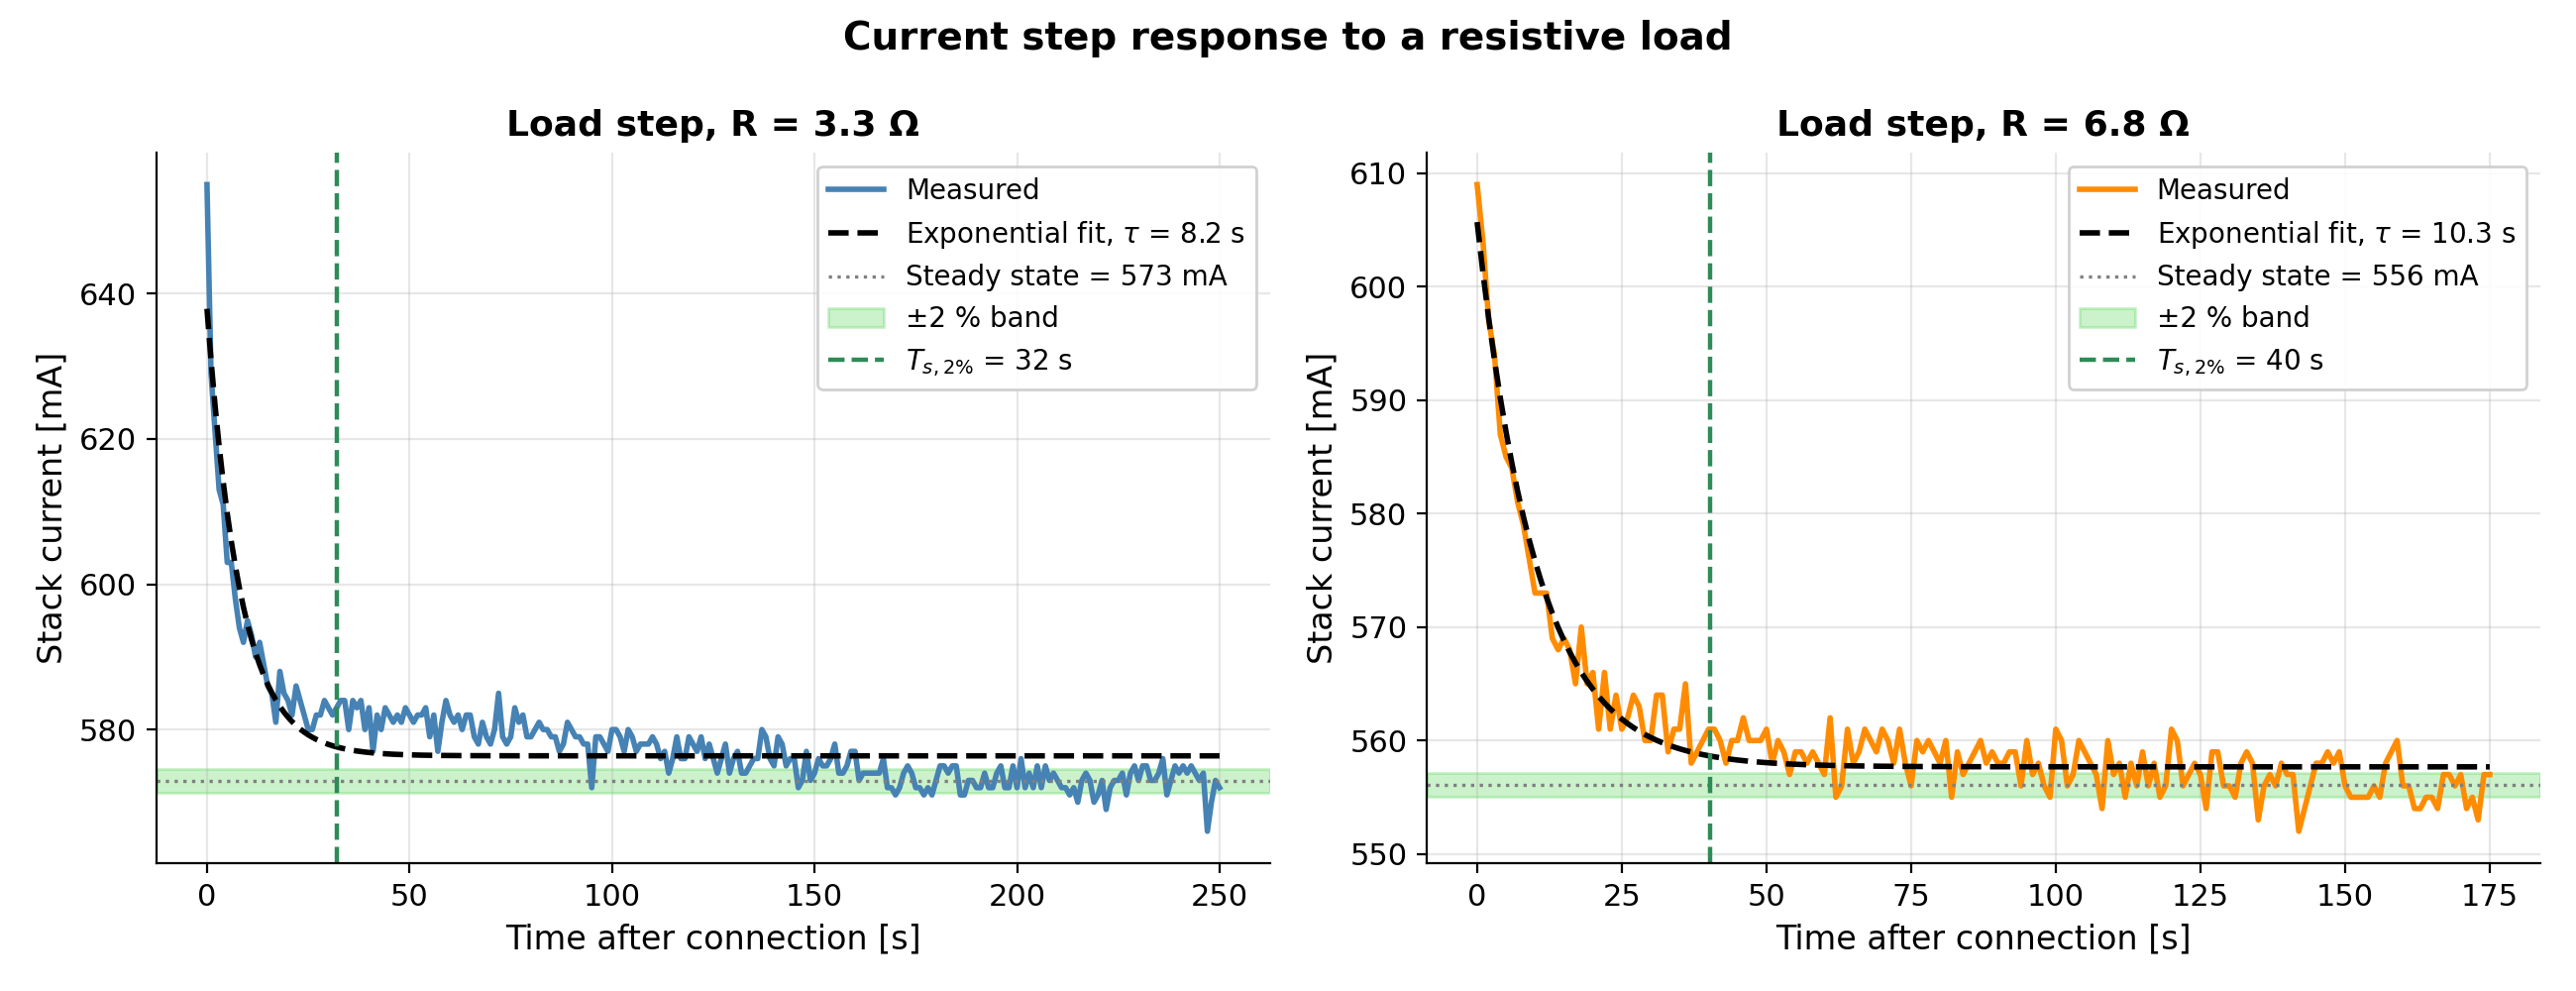
\includegraphics[width=0.95\linewidth]{Figures/response_time_plot.png}
    \caption[Current step response and exponential fit]{Current step response for
             the two loads: measured current (color), exponential fit (dashed),
             steady-state level, $\pm2\,\%$ settling band, and the 2\,\% settling
             time. The exponential model matches the data closely, justifying the
             first-order time constants reported in Table~\ref{tab:response-rt}.}
    \label{fig:tr-responses}
\end{figure}

The current time constant is about 25\,\% longer under the lighter load
($\tau_I=10.3$\,s at $6.8\,\Omega$ versus $8.2$\,s at $3.3\,\Omega$), consistent
with slower electrochemical dynamics at lower current density; the initial
perturbation $\Delta I$ is also smaller (52.9 versus 82.1\,mA). The settling times
derived from the fit ($T_{s,2\%}=32$--$40$\,s) are robust to measurement noise,
because they are computed analytically from $\tau_I$ rather than read off the
noisy raw signal. This timescale captures the dominant dynamics seen by the load
--- electrochemical kinetics combined with gas-supply transients --- and sets a
quantitative target for controller bandwidth: the closed-loop controller of
Chapter~\ref{Chapter5} must act well within $\tau_I\approx 8$--$10$\,s to shape the
stack's transient behavior.
